\section{Обзорный раздел по предметной области}

\subsection{Использование формул}



Ненумерованная формула:

\begin{equation}
    \begin{pmatrix} \dot{\varphi}\\ \dot{\theta} \\ \dot{\psi} \end{pmatrix}
    = \begin{pmatrix}
        cos(\theta)cos(\psi) & -sin(\psi) & 0 \\
        cos(\theta)sin(\psi) & cos(\psi)  & 0 \\
        -sin(\theta)         & 0         &  1
    \end{pmatrix}^{-1}
    \begin{pmatrix} \omega_x\\ \omega_y \\ \omega_z \end{pmatrix}.
\end{equation}

Нумерованная формула:

\begin{equation}
    i^2 = -1.
    \label{eq:my_ref}
\end{equation}

Тест ссылки на формулу \ref{eq:my_ref}.

\subsection{Вставка рисунков}

\begin{figure}[ht]
\begin{center}
\scalebox{0.4}{
   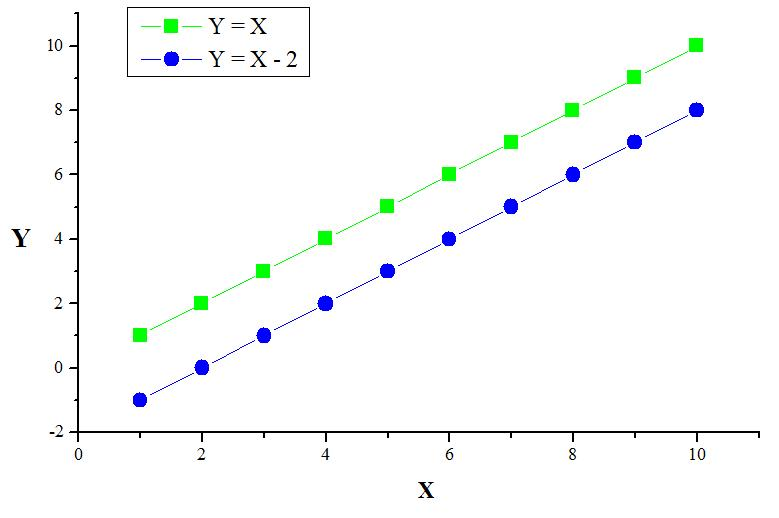
\includegraphics{images/graph.jpg}
}

\caption{
\label{graph-fig}
     Линейные функции.}
\end {center}
\end {figure}
Ссылаемся на график~\ref{graph-fig}.

\subsection{Ссылки на источники}

Ссылки на источники: \cite{voc}, \cite{vo2}, \cite{ij-sdk}.

\subsection{Оформление фрагментов кода}

В работах иногда приводят фрагменты кода:

\begin{minted}{kotlin}
fun main() {
    val name = "stranger"
    println("Hi, $name!")
    print("Current count:")
    for (i in 0..10) {
        print(" $i")
    }
}
\end{minted}


\subsection{Оформление таблиц}


\begin{table}[ht]
\begin{center}
\begin{tabular}{lccc}
    Имя & Работа 1 & Работа 2 & Итог \\
\hline
    Алиса & 8.0 & 9.0 & 8.5 \\
    Боб & 9.0 & 9.8 & 9.4 \\
    Чак & 9.1 & 9.3 & 9.2 \\
\end{tabular}
\caption{
\label{table-smth}
     Сравнение результатов.}
\end {center}
\end {table}

Ссылаемся на таблицу~\ref{table-smth}.


